\documentclass[tikz, border=-1cm]{standalone}
\usetikzlibrary{decorations.markings}

\RequirePackage{tikz, pgfplots,
                tikz-3dplot, tkz-euclide}  % TikZ tegner figurer, og PGFPlots er godt verktøy for plotting
    \usetkzobj{all} % Brukt av tikz-euclide, f.eks for mangekanter, og andre % geometriske figurer
    \usetikzlibrary{calc}                   % calc-biblioteket til TikZ
    \usetikzlibrary{decorations.markings}   % decorations-biblioteket til TikZ
    \pgfplotsset{compat=newest}             % Unngå kompabilitetserror fra PGFPlots
    \usetikzlibrary{angles,patterns}


% Defines a style to produce arrows along an arbitary curve
%
% Usage:
% draw plot ... [arrow inside={end=stealth,opt={scale=2}}{0.25,0.5,0.75}];'
\tikzset{
    set arrow inside/.code={\pgfqkeys{/tikz/arrow inside}{#1}},
    set arrow inside={end/.initial=>, opt/.initial=},
    /pgf/decoration/Mark/.style={
        mark/.expanded=at position #1 with
        {
            \noexpand\arrow[\pgfkeysvalueof{/tikz/arrow inside/opt}]{\pgfkeysvalueof{/tikz/arrow inside/end}}
        }
    },
    arrow inside/.style 2 args={
        set arrow inside={#1},
        postaction={
            decorate,decoration={
                markings,Mark/.list={#2}
            }
        }
    },
}

\usepackage{pgfplots}

\begin{document}
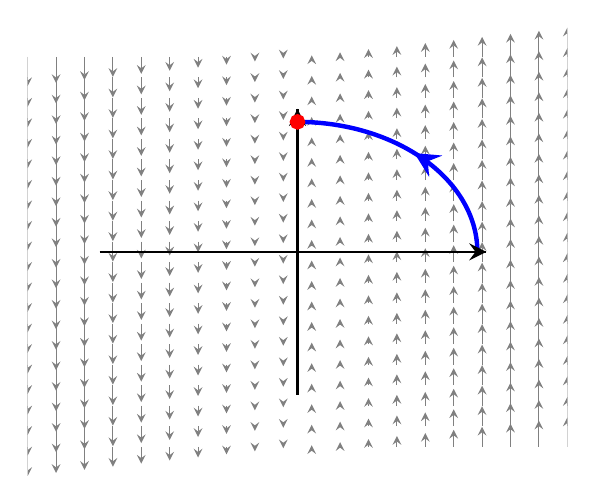
\begin{tikzpicture}
  \begin{axis}[domain=-1.5:1.5, view={0}{90}, axis lines = none, legend style =
    {at={(0,1)}, anchor=north west, draw = none}, ]
    \addplot3[gray, quiver={u={0}, v={x}, scale arrows=0.15},
    -stealth,samples=20, empty legend] {0};

    \addplot [domain=0:90, samples=100, ultra thick, color=blue]
    ({cos(x)},{sin(x)}) [arrow inside={end=stealth
      ,opt={blue,scale=1.5}}{0.5}];

    \addplot [domain=-1.1:1.05, samples=100, thick, color=black]
    ({x},{0}) [arrow inside={end=stealth
      ,opt={black,scale=1.5}}{1}];

        \addplot [domain=-1.1:1.1, samples=100, thick, color=black]
    ({0},{x}) [arrow inside={end=stealth
      ,opt={black,scale=1.5}}{1}];

    \addplot[color=red, mark=*, ultra thick] coordinates {(0,1)};
  \end{axis}


  % \coordinate (P) at (5.4,2.85); \filldraw (P) circle[radius=3pt]; \node[above
  % right=5pt of {P}, outer sep=2pt,fill=white] {P};

  % \coordinate (Q) at (1.43,2.85); \filldraw (Q) circle[radius=3pt]; \node[above
  % left=5pt of {Q}, outer sep=2pt,fill=white] {Q};
\end{tikzpicture}%
\end{document}